% Basic LaTeX template for NE 204 lab report
\documentclass[11pt]{article}

%==============================================================================
%%% Everything between the "="'s is the preamble.
%%% Define packages and meta data here

% Common packages
\usepackage{amsmath}    % Expanded math
\usepackage{amssymb}    % Expanded math symbols
\usepackage{graphicx}   % For images
%\usepackage[version=3]{mhchem} % For nuclide formatting

% All images/figures will be stored in the images folder.
% Specify that here so pdflatex knows where to look for images.
\graphicspath{{./images/}}

% Metadata
\title{Lab Report Template}
\author{Ross Barnowski}
\date{\today}
%==============================================================================

\begin{document}

% Compile metadata from preamble into a nicely-rendered title section
\maketitle

% The *'s next so section/subsection definitions suppresses numbering
\section*{Introduction}
\label{sec:intro}
%Introduction / motivation / background go here.
Peak fitting is a fundamental and essential exercise for conducting gamma ray spectroscopy.
The ability to take raw data from a detector and turn it in to the initial stage of usable
data is a task all individuals studying nuclear science should know and understand. We first begin to
understand the information contained in each particle by determining its energy.  The methods to make this
determination vary, but for this lab a HPGe detector with a 13-bit resolution MCA, producing 8192 bin spectra was used.
Through proper analysis and manipulation of this data, a wealth of information can be determined.
This lab facilitated the usage of modern data analysis techniques to take gamma ray energy data from
multiple sources and conduct an energy calibration.

\subsection*{Motivation}
\label{sec:motivation}

The purpose of this report has three key elements:

\begin{enumerate}
  \item To learn how to write lab reports using \LaTeX and the NE 204 template.
  \item To learn to use {\tt numpy} and {\tt scipy} to fit models to data.
  \item Te lean how to collaborate with others in the field to achieve a common goal.
\end{enumerate}

Each one of these elements, will better prepare us to undertake for advanced experiments in the future.
The ability to properly manage and store data, as well as to collaborate with our peers can not be overlooked.


\section*{Methods}
\label{sec:meth}
Experimental procedure / set up / methods go here.


\section*{Results}
\label{sec:res}

Using a linear fit from the energy calibration earlier, we applied this to the $^{133}$Ba data to yield the
plot below.

\begin{figure}[H]
  \begin{center}
    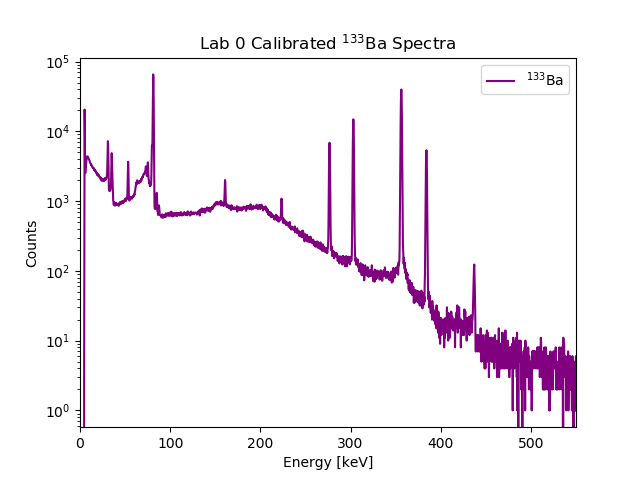
\includegraphics[width=10cm]{ba_calibrated.png}
    \caption{\label{fig:ba133}Calibrated $^{133}$Ba Spectra}
  \end{center}
\end{figure}

The accepted values were then compared against the energy values found thought the energy calibration, calculating the
percent difference between the two.
\\

\begin{tabular}{lll}
\toprule
Calculated Energy [keV] & Accepted Value [keV] & Precent Difference \% \\
\midrule
     81.14525+/-0.00010 &     80.9979+/-0.0011 &      0.1819+/-0.0014 \\
    356.39031+/-0.00005 &    356.0129+/-0.0007 &    0.10601+/-0.00020 \\
      5.10916+/-0.00011 &                 4.47 &     14.2988+/-0.0024 \\
    303.08087+/-0.00006 &    302.8508+/-0.0005 &    0.07597+/-0.00017 \\
     30.92215+/-0.00010 &               32.194 &    3.95059+/-0.00033 \\
    276.70673+/-0.00006 &      275.925+/-0.007 &      0.2833+/-0.0025 \\
    384.16733+/-0.00005 &    383.8485+/-0.0012 &    0.08306+/-0.00031 \\
\bottomrule
\end{tabular}

\\

This comparison shows that the linear fit is good for higher gamma energies but is significantly
degraded for lower energy events.


\section*{Discussion}
\label{sec:disc}
Energy calibration is a tedious but necessary step in nuclear data analysis. In future code,
the ability to link the calibration files to set databases or to even automate the selection of known energies
would greatly speed up the calibration process.  With our method, there persists a requirement to manually
enter values into the script before energy calibration is conducted. The reproducibility of this process is a valuable
tool moving forward and will improve our ability to process data.  


% Bibliography
\bibliographystyle{plain}
% Refers to a bibtex file in the current dir named "references.bib"
\bibliography{references}

\end{document}
